\documentclass[12pt,a4paper]{article}

\usepackage[utf8]{inputenc}
\usepackage[T1]{fontenc}
\usepackage[brazil]{babel}
\usepackage{times}
\usepackage{geometry}
\usepackage{graphicx}
\usepackage{booktabs}
\usepackage{array}
\usepackage{float}
\usepackage{url}
\usepackage{amsmath}
\usepackage{caption}

\geometry{
  left=3cm,
  right=3cm,
  top=3cm,
  bottom=2.5cm
}

\captionsetup{font=small,labelfont=bf}
\setlength{\parindent}{1.25cm}
\setlength{\parskip}{0pt}

\title{\textbf{Relat\'orio da Atividade 2 -- Etapa 3: Captura e An\'alise do Tr\'afego CAN}}

\author{
\'Alvaro C. Negromonte\textsuperscript{1},
Victoria Pessoa Barbosa Matos\textsuperscript{1},
Pedro C. Guimar\~aes Rodrigues\textsuperscript{1}
\\[0.3cm]
\textsuperscript{1}Centro de Inform\'atica -- Universidade Federal de Pernambuco (CIn/UFPE)
\\
IF747 -- Redes Automotivas -- 2026.1
\\
Recife -- PE -- Brasil
\\
\texttt{[acn3, vpbm, pcgr]@cin.ufpe.br}
}

\date{}

\begin{document}

\maketitle

\noindent\textbf{Resumo.}
Este relat\'orio apresenta a captura e a an\'alise do tr\'afego CAN gerado no ambiente
Yes, CARLA CAN durante dois cen\'arios experimentais: opera\c{c}\~ao normal do
ve\'iculo e execu\c{c}\~ao de um ataque de \textit{spoofing} sobre a fun\c{c}\~ao de freio de
m\~ao. A etapa utilizou o arquivo DBC customizado criado na Etapa 2, mantendo os
identificadores e per\'iodos de transmiss\~ao definidos anteriormente. Foram coletados
logs com \texttt{candump}, processadas estat\'isticas por ID CAN e gerados gr\'aficos
comparativos. Os resultados mostram aumento expressivo no tr\'afego do ID \texttt{0x604}
durante o ataque, acompanhado de impacto visual no simulador: o ve\'iculo deixou de
se mover enquanto o \textit{spoofing} estava ativo.

\section{Introdu\c{c}\~ao}

A terceira etapa da atividade teve como objetivo capturar e comparar o tr\'afego CAN
do ve\'iculo simulado em dois cen\'arios distintos. No primeiro, o ve\'iculo foi operado
normalmente no ambiente Yes, CARLA CAN. No segundo, foi executado um ataque de
\textit{spoofing} sobre uma fun\c{c}\~ao veicular, com o objetivo de injetar mensagens
maliciosas no barramento virtual \texttt{vcan0}.

O experimento d\'a continuidade \`a Etapa 2, na qual foi criado um arquivo DBC
customizado para a rede CAN virtual. Esse arquivo foi utilizado novamente nesta etapa
para garantir consist\^encia entre a configura\c{c}\~ao da rede, os IDs CAN observados e a
an\'alise dos logs capturados.

\section{Configura\c{c}\~ao Experimental}

O ambiente foi executado a partir do reposit\'orio Yes, CARLA CAN, utilizando o
arquivo \texttt{data/our\_dbcfile.dbc}. O comando usado para inicializar a plataforma foi:

\begin{verbatim}
./1_up_environment.sh --dbc data/our_dbcfile.dbc
\end{verbatim}

O DBC customizado possui sete mensagens peri\'odicas, incluindo as cinco mensagens
principais modificadas na Etapa 2 e duas mensagens auxiliares necess\'arias para a
compatibilidade com a plataforma. A Tabela~\ref{tab:dbc} resume os IDs e per\'iodos
utilizados.

\begin{table}[H]
\centering
\caption{Mensagens do DBC customizado utilizadas no experimento.}
\label{tab:dbc}
\begin{tabular}{lcc}
\toprule
\textbf{Mensagem} & \textbf{ID CAN} & \textbf{Per\'iodo} \\
\midrule
THROTTLE & \texttt{0x710} & 50 ms \\
BRAKE & \texttt{0x711} & 200 ms \\
STEER & \texttt{0x712} & 50 ms \\
GEAR & \texttt{0x713} & 200 ms \\
REVERSE & \texttt{0x714} & 200 ms \\
HAND\_BRAKE & \texttt{0x604} & 200 ms \\
MANUAL\_TRANSMISSION & \texttt{0x606} & 500 ms \\
\bottomrule
\end{tabular}
\end{table}

\section{Captura do Tr\'afego CAN}

As capturas foram realizadas com a ferramenta \texttt{candump}, registrando as mensagens
transmitidas no barramento virtual \texttt{vcan0}. Foram gerados dois arquivos de log:

\begin{itemize}
    \item \texttt{normal.log}: captura durante opera\c{c}\~ao normal do ve\'iculo;
    \item \texttt{spoofing\_hand\_brake.log}: captura durante ataque de \textit{spoofing}
    sobre a fun\c{c}\~ao de freio de m\~ao.
\end{itemize}

O comando utilizado para a captura foi:

\begin{verbatim}
candump -l vcan0
\end{verbatim}

No cen\'ario normal, o arquivo capturado possui 3954 linhas. No cen\'ario com ataque,
o arquivo capturado possui 5921 linhas. A diferen\c{c}a j\'a indica aumento na quantidade
total de mensagens transmitidas durante o per\'iodo analisado.

\section{Ataque de Spoofing}

O ataque escolhido foi o \textit{spoofing} da fun\c{c}\~ao \texttt{hand\_brake}, que injeta
mensagens no ID CAN \texttt{0x604}. Esse ID foi mantido no DBC customizado da Etapa 2,
o que torna o ataque compat\'ivel com a configura\c{c}\~ao atual da rede.

O comando utilizado foi:

\begin{verbatim}
conda run --no-capture-output -n n4s_env python3 cyberattacks_module.py \
  --feature hand_brake --period 0.01
\end{verbatim}

O per\'iodo de 0,01 s corresponde a uma tentativa de transmiss\~ao de aproximadamente
100 mensagens por segundo pelo m\'odulo de ataque. Durante a execu\c{c}\~ao do
\textit{spoofing}, foi observado no simulador CARLA que o ve\'iculo n\~ao conseguia se
mover, mesmo com comandos de acelera\c{c}\~ao. Esse comportamento \'e consistente com
a inje\c{c}\~ao repetida de mensagens que ativam o freio de m\~ao.

\begin{figure}[H]
\centering
\fbox{\begin{minipage}[c][4.2cm][c]{0.9\linewidth}
\centering
Inserir aqui uma captura extra\'ida do v\'ideo do cen\'ario normal.
\end{minipage}}
\caption{Opera\c{c}\~ao normal do ve\'iculo no CARLA.}
\label{fig:video-normal}
\end{figure}

\begin{figure}[H]
\centering
\fbox{\begin{minipage}[c][4.2cm][c]{0.9\linewidth}
\centering
Inserir aqui uma captura extra\'ida do v\'ideo durante o ataque de \textit{spoofing}.
\end{minipage}}
\caption{Ataque de \textit{spoofing} de freio de m\~ao: o ve\'iculo n\~ao se move durante a inje\c{c}\~ao das mensagens.}
\label{fig:video-spoofing}
\end{figure}

\section{An\'alise Quantitativa}

Os logs foram processados com o script \texttt{data/can\_bus\_data\_analyzer.py}, gerando
estat\'isticas por ID CAN e gr\'aficos comparativos. A Tabela~\ref{tab:comparacao}
apresenta os principais resultados obtidos.

\begin{table}[H]
\centering
\caption{Compara\c{c}\~ao da quantidade de mensagens por ID CAN.}
\label{tab:comparacao}
\begin{tabular}{lrrrr}
\toprule
\textbf{ID CAN} & \textbf{Normal} & \textbf{Spoofing} & \textbf{Dif.} & \textbf{Taxa no ataque} \\
\midrule
\texttt{0x604} & 365 & 3002 & 2637 & 49,22 msg/s \\
\texttt{0x606} & 148 & 120 & -28 & 1,97 msg/s \\
\texttt{0x710} & 1186 & 962 & -224 & 15,69 msg/s \\
\texttt{0x711} & 365 & 294 & -71 & 4,82 msg/s \\
\texttt{0x712} & 1186 & 962 & -224 & 15,69 msg/s \\
\texttt{0x713} & 339 & 287 & -52 & 4,71 msg/s \\
\texttt{0x714} & 365 & 294 & -71 & 4,82 msg/s \\
\bottomrule
\end{tabular}
\end{table}

O resultado mais relevante ocorre no ID \texttt{0x604}, associado \`a mensagem
\texttt{HAND\_BRAKE}. No cen\'ario normal, foram observadas 365 mensagens nesse ID,
com taxa aproximada de 4,82 mensagens/s e per\'iodo m\'edio de 208 ms. Durante o
ataque, foram observadas 3002 mensagens no mesmo ID, com taxa aproximada de
49,22 mensagens/s e per\'iodo m\'edio de 20,32 ms. A diferen\c{c}a de 2637 mensagens
representa o efeito direto da inje\c{c}\~ao realizada pelo m\'odulo de ataque.

\begin{figure}[H]
\centering
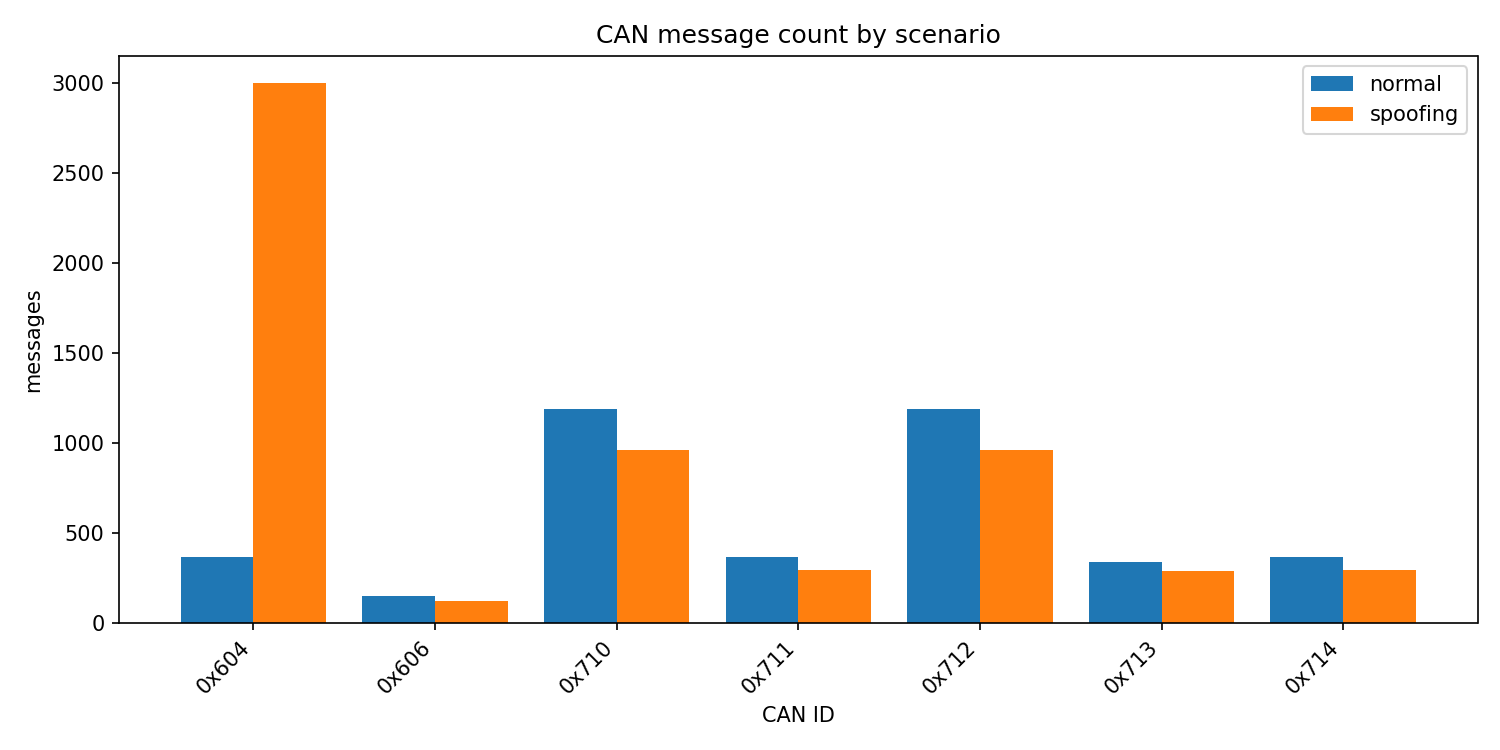
\includegraphics[width=0.95\linewidth]{figures/message_counts_by_id.png}
\caption{Quantidade de mensagens por ID CAN nos cen\'arios normal e com \textit{spoofing}.}
\label{fig:counts}
\end{figure}

A Figura~\ref{fig:counts} mostra que o ID \texttt{0x604} domina a diferen\c{c}a entre os
dois cen\'arios. Os demais IDs permanecem com taxas pr\'oximas \`as esperadas para seus
per\'iodos de transmiss\~ao, com diferen\c{c}as atribu\'idas principalmente \`a dura\c{c}\~ao
ligeiramente diferente das capturas.

\begin{figure}[H]
\centering
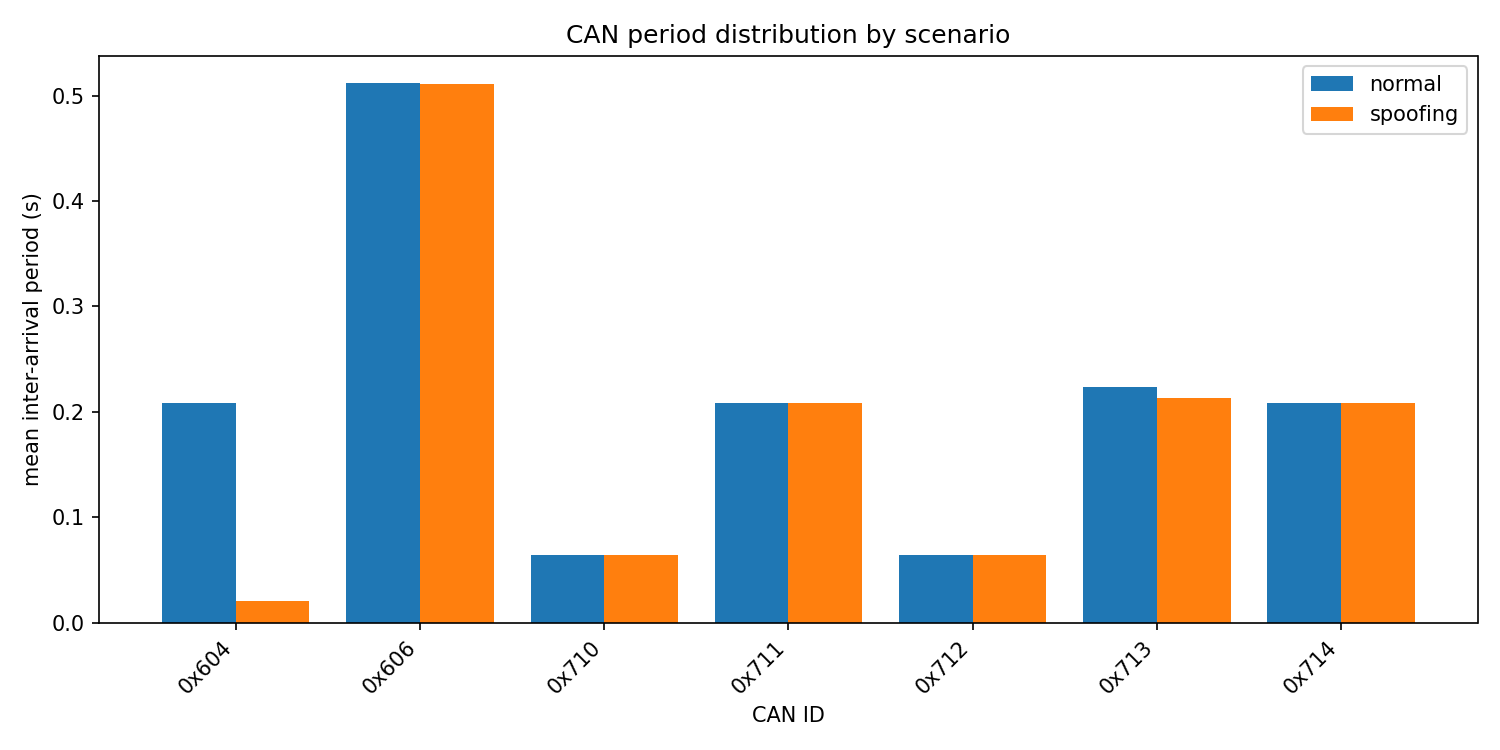
\includegraphics[width=0.95\linewidth]{figures/mean_period_by_id.png}
\caption{Per\'iodo m\'edio entre mensagens por ID CAN nos cen\'arios analisados.}
\label{fig:periods}
\end{figure}

A Figura~\ref{fig:periods} evidencia a redu\c{c}\~ao do per\'iodo m\'edio do ID
\texttt{0x604}. O per\'iodo cai de aproximadamente 208 ms para 20 ms durante o ataque.
Essa redu\c{c}\~ao altera o padr\~ao temporal esperado para a mensagem de freio de m\~ao
e cria uma assinatura clara de comportamento an\^omalo no barramento CAN.

\section{Discuss\~ao}

O experimento mostrou que a aus\^encia de autentica\c{c}\~ao nas mensagens CAN permite
que um n\'o malicioso injete frames com o mesmo ID de uma fun\c{c}\~ao veicular leg\'itima.
Como os receptores interpretam as mensagens com base no ID e no formato definido no
DBC, a mensagem falsa de \texttt{HAND\_BRAKE} foi aceita pela plataforma como uma
mensagem v\'alida.

Do ponto de vista quantitativo, o ataque foi facilmente observ\'avel pela eleva\c{c}\~ao
da taxa de mensagens no ID \texttt{0x604}. Do ponto de vista veicular, o impacto tamb\'em
foi claro: durante o \textit{spoofing}, o ve\'iculo n\~ao conseguia se deslocar porque o freio
de m\~ao era continuamente for\c{c}ado pelo tr\'afego injetado.

Esse comportamento demonstra uma vulnerabilidade central do protocolo CAN: a rede
foi projetada para comunica\c{c}\~ao eficiente e determin\'istica entre ECUs, mas n\~ao
inclui mecanismos nativos de autentica\c{c}\~ao, autoriza\c{c}\~ao ou integridade das
mensagens. Assim, se um atacante obtiver acesso ao barramento, ele pode interferir em
fun\c{c}\~oes veiculares por meio de mensagens bem formatadas.

\section{Conclus\~ao}

A Etapa 3 foi conclu\'ida com a captura e an\'alise de dois cen\'arios de tr\'afego CAN:
opera\c{c}\~ao normal e ataque de \textit{spoofing} sobre o freio de m\~ao. Os logs
capturados com \texttt{candump} foram analisados por ID CAN, permitindo comparar
contagens, taxas de mensagens e per\'iodos m\'edios.

Os resultados mostraram aumento expressivo no ID \texttt{0x604}, que passou de 365
mensagens no cen\'ario normal para 3002 mensagens durante o ataque. A taxa do ID
subiu de aproximadamente 4,82 mensagens/s para 49,22 mensagens/s, enquanto o per\'iodo
m\'edio caiu de 208 ms para 20 ms. Esse resultado confirma que o ataque alterou de forma
mensur\'avel o padr\~ao temporal da rede CAN.

Al\'em da diferen\c{c}a quantitativa, o impacto no comportamento do ve\'iculo tamb\'em
foi observado no simulador CARLA: durante o \textit{spoofing}, o ve\'iculo ficou impedido
de se mover. Portanto, o experimento evidencia a relev\^ancia de mecanismos de detec\c{c}\~ao
e mitiga\c{c}\~ao de intrus\~oes em redes intraveiculares baseadas em CAN.

\end{document}
